\section{Movimiento y posicionamiento en interiores}

El control del movimiento y posicionamiento requiere procedimientos robustos que integren estrategias de planificación y ejecución en tiempo real.

Para que el robot se mueva por medio de sus ruedas, se utilizan controladores PID (Proporcional, Integral y Derivativo), los cuales ajustan dinámicamente las velocidades de las ruedas. Por otro lado, los sistemas más avanzados pueden integrar estrategias de Control Predictivo por Modelo (MPC), optimizando la trayectoria del robot mediante predicciones basadas en el modelo cinemático. Adicionalmente, el robot debe incorporar sensores para la retroalimentación del movimiento, como encoders en las ruedas y acelerómetros. Esta información es utilizada para ajustar y corregir el control en tiempo real.

Los algoritmos de control, como los basados en PID (Proporcional, Integral y Derivativo) o MPC (Control Predictivo por Modelo), permiten ajustar las velocidades y trayectorias del robot de manera precisa para evitar colisiones y garantizar estabilidad. Además, la navegación en interiores puede beneficiarse de técnicas como la SLAM (Simultaneous Localization and Mapping), que combina la localización con la construcción de mapas del entorno, ofreciendo una representación dinámica y actualizada. Cabe destacar la existencia de estimadores de estado genéricos como ser Filtro de Kalman, que permite la fusión de datos de múltiples sensores.

En la actualidad, los sistemas de posicionamiento en interiores (IPS, por sus siglas en inglés) se han convertido en una herramienta esencial en la navegación en espacios cerrados. La implementación de estas tecnologías puede lograrse mediante el uso de balizas de radiofrecuencia (Bluetooth, Wi-Fi, banda ultra ancha UWB), ultrasonido, etiquetas RFID y comunicaciones por luz visible (VLC, por sus siglas en inglés). \cite{nuaimisurveyindoorpositioning}

A pesar de los avances logrados, el posicionamiento asistido por GPS en interiores presenta limitaciones significativas debido a la gran pérdida de trayectoria provocada por las paredes de los edificios. Este debilitamiento de la señal lo convierte en una opción poco viable en comparación con otras tecnologías más especializadas.

Por otro lado, el uso de ultrasonido presenta problemas derivados de la alta atenuación en el aire, lo que dificulta su aplicación en eventos que requieran un amplio alcance. Otros métodos de posicionamiento, como infrarrojos, Zigbee y Bluetooth, aunque prometedores, pueden ser vulnerables a fluctuaciones en las fuentes de señal. No obstante, esta limitación podría mitigarse a través de soluciones como la implementación de una granja de antenas para garantizar una señal estable. En términos de precisión, las tecnologías tradicionales como Wi-Fi, Bluetooth y RFID activo proporcionan una precisión que generalmente varía en el rango de varios metros.

En cuanto a las comunicaciones de luz visible (VLC), se destacan por su enfoque innovador al detectar luz mediante fotodetectores. El uso de un único detector permite realizar una lateralización circular, mientras que la implementación de dos detectores habilita un posicionamiento diferencial. Este último método ha demostrado un mejor desempeño y una mayor reducción en el margen de error, consolidándose como una solución prometedora para futuros desarrollos tecnológicos en el ámbito del posicionamiento en interiores.

Cambien podemos mencionar los seguidores de línea, que representan un ejemplo simplificado de navegación basada en detección. Se emplean sensores para identificar y seguir líneas o patrones, que actúan como guías para el control del movimiento y la localización en entornos estructurados.

A continuación se detalla una tabla comparativa sobre las diferentes alternativas para posicionamiento en interiores, entre ellos, los distintos sistemas de localización en tiempo real que existen, también conocidos como RTLS \cite{alammarsurveyindoor}.

\begin{figure}[H]
    \centering
    \hspace*{-1.0cm}
    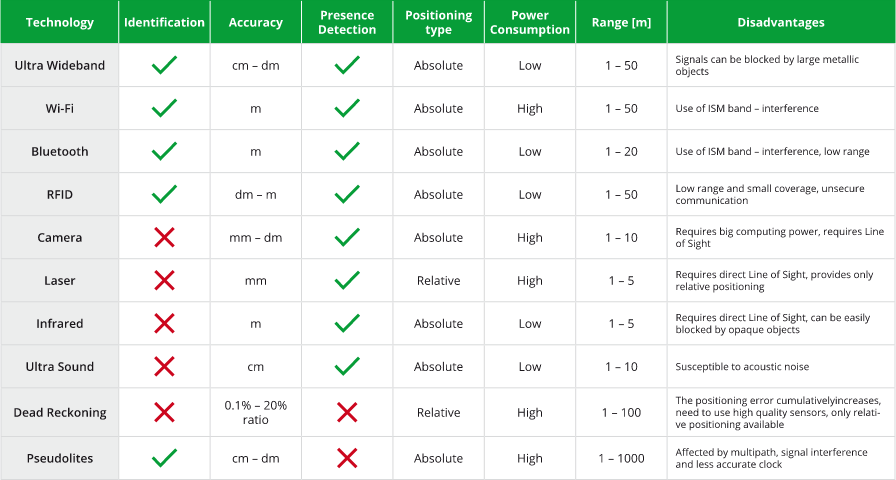
\includegraphics[width=1.1\linewidth]{mt_RTLS_comparacion}
    \caption{Comparativa entre métodos de posicionamiento en interiores}
    \label{fig:compmetposindor}
\end{figure}


\subsection{Filtro de Kalman}

El filtro de Kalman constituye una herramienta esencial en la robótica para la estimación del estado de un sistema dinámico en entornos sujetos a incertidumbre y ruido en las mediciones. En el caso de robots omnidireccionales, su aplicación es particularmente útil para determinar la posición de un objeto en tiempo real mediante la integración de datos provenientes de múltiples sensores. Este proceso permite superar las limitaciones impuestas por el ruido inherente y las diferencias en las frecuencias de muestreo de los sensores.

El funcionamiento del filtro de Kalman se fundamenta en dos etapas principales: la predicción y la actualización. En la fase de predicción, se estima el estado del sistema y su incertidumbre utilizando modelos cinemáticos que describen el movimiento del objeto. En la etapa de actualización, las observaciones obtenidas de los sensores se incorporan para ajustar la estimación, ponderando cada medición según su nivel de precisión. Este enfoque posibilita la integración eficaz de entradas provenientes de sensores como cámaras, acelerómetros, encoders, entre otros, incluso cuando las frecuencias de muestreo difieren entre sí. \cite{nuaimisurveyindoorpositioning}


\subsection{Detección y medición de QR}

La detección y utilización de códigos QR en la robótica interior han demostrado ser una solución económica y eficiente para la navegación y localización del robot. Estos códigos, colocados en paredes y áreas visibles, pueden almacenar información relevante sobre el entorno, como la sección o ubicación específica dentro del espacio. Además, su bajo costo de producción los hace ideales para proyectos de robótica en interiores. \cite{tzafestas2013introduction}

La lectura de los códigos QR se realiza mediante cámaras integradas en el robot. Estas cámaras capturan imágenes del código y, utilizando técnicas de procesamiento de imagen, decodifican la información almacenada. Además, se puede estimar la distancia entre el robot y el código QR con un nivel razonable de precisión, aprovechando el tamaño conocido del código y las características del encuadre de la cámara. Este cálculo, basado en principios de geometría proyectiva, permite al robot ajustar su posición y orientar sus movimientos en función de los datos obtenidos.
